\documentclass[11pt]{article}
\usepackage{geometry}                % See geometry.pdf to learn the layout options. There are lots.
\geometry{letterpaper}                   % ... or a4paper or a5paper or ... 
%\geometry{landscape}                % Activate for rotated page geometry
\usepackage[parfill]{parskip}    % Activate to begin paragraphs with an empty line rather than an indent
\usepackage{graphicx}
\usepackage{amssymb}
\usepackage{amsmath}
\usepackage{epstopdf}
\usepackage{ulem}
\usepackage[colorlinks]{hyperref} %allows for links, e.g. \href{<url>}{<text>}
%\DeclareGraphicsRule{.tif}{png}{.png}{`convert #1 `dirname #1`/`basename #1 .tif`.png}

\title{Project Plan}
\author{Team Orange}
\date{\today}

\begin{document}

\begin{centering}
\textbf{\huge{Android dotCal}}\\
\LARGE{Project Plan}

\end{centering}

%\title
%\tableofcontents

\vspace{1cm}
\textbf{\large{Version History}}

\begin{tabular}{|l|l|l|c|}
\hline
Version Number & Authors & Description & Date\\
\hline
Version 1 & Team Orange & The Initial Version & 12/8 \\
\hline
\end{tabular}\\\\

\textbf{\large{Review History}}

\begin{tabular}{|l|l|l|c|}
\hline
Reviewed By & Version & Comments & Date\\
\hline
Kelsey & 0 & Did not exist yet & 11/23 \\
\hline
Kelsey & 1 & Just integrated everyone's segments & 12/8\\
\hline
\end{tabular}\\\\

\textbf{\large{Approvals}}

\begin{tabular}{|l|l|l|c|}
\hline
Approved By & Version & Signature & Date\\
\hline
Kelsey & 1 & \hspace{2in} & 12/8 \\
\hline
\end{tabular}


\section{Overview}

neutralSpace has invented an application platform called dotCal which they define as one that �creates tools that free people�s time management from the constraints of a single device, operating system or corporate network.�  The application we are developing is designed to be a part of the dotCal platform and run on the T-Mobile's G1 Android mobile phone.  The purpose of this application is to easily let the user track where they were and when. The user starts an event with a single click. The phone should then automatically find its location. When the user is done with their activity, they can click ``Stop," and their location and time spent there will be logged as a calendar entry. 

With future versions, the recorded information will be publishable to the web. The intent is to help automate facebook and Twitter-like social networking status updates and blogging.

\section{Deliverables}
Installable Android Package (APK) along with a 1.0 tagged source tree in the source control repository.
\section{Assumptions, Constraints and References}
	The team assumes that:
	\begin{itemize}
	\item The application will run on the ``T-Mobile G1" Android-platform phone
	\item Any updates published by Google to
		\begin{itemize}
		\item Android SDK,
		\item Android Operating System,
		\item Android Calendar API,
		\item Google Calendar Web API, or
		\item Android Marketplace
		\end{itemize}
		during the application's development will be inconsequential to the schedule and system architecture
	\item neutralSpace will use Eclipse to build the application, or will nonetheless find satisfactory the team providing Eclipse Project and Ant build scripts
	\end{itemize}

\section{Development Process}
\begin{enumerate}
 \item \textbf{Establish customer needs.} \textit{Everyone} will meet with neutralSpace (nS) and determine overall purpose of application and expected functionality. (\underline{Complete})
 \item \textbf{Write needs down in the form of a Requirements Document.} \textit{Kelsey} and \textit{Adam} will develop a concise list of detailed program requirements. \textit{Sky} will create a Visio document reflecting these needs with wireframes and mockups of the application screens, along with the program flow. (\underline{Complete})
 \item \textbf{Customer approval of needs.} \textit{Everyone} will present the Requirements/Visio document to nS for review and incorporate any corrections they have into the document. (\underline{Complete})
 \item \textbf{Create system architecture.} \textit{Armando}, \textit{Sky}, and \textit{Adam} will meet together and split the requirements into concrete components/modules that can be developed separately by multiple team members at once. \textit{Everyone except Nathan} has secondary roles as developers, so these members will be potential assignees for implementing these modules. (\underline{By January 1, 2009})
 \item \textbf{Code the components.} Members with roles as developers will be assigned a component, with the larger and more complex components (e.g. Calendar syncing) being implemented by \textit{Armando}. (\underline{Ongoing before February 21, 2009})
 \item \textbf{Test each component.} Each component will have unit tests that will be developed by the component author. (\underline{Ongoing before February 21, 2009})
 \item \textbf{Integrate components.} As individual components are completed, they can interact with other completed components eventually forming the overall application. (\underline{Ongoing before February 21, 2009})
 \item \textbf{Test integrated system.} All components should be working together as expected, at this point QA can do a final sweep of functional tests and system tests allowing a week of final bug fixing and polishing before the initial release. (\underline{February 21, 2008})
\end{enumerate}


\section{PERT Chart}

\includegraphics[scale=.5]{Capstone_Pert}


\section{Schedule}
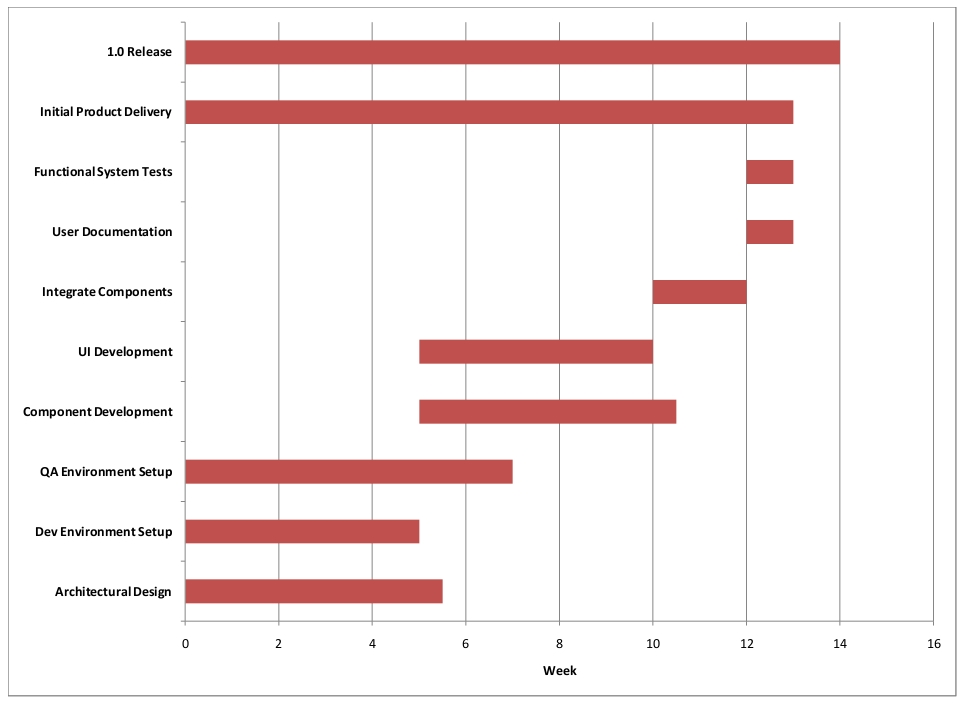
\includegraphics[scale=.7]{Capstone_PP_Gantt}

%\section{Calendar}
\section{Meetings and Reviews}
We will have a team meeting every-other week just to keep each other informed and address any issues we may have encountered.  We will invite neutralSpace to join us for the first and last meetings of winter term.  But, after that, meetings with neutralSpace will be done on an as-needed basis.

\section{Resource Identification}
	Summary of resources identified:
	\begin{itemize}
		\item{T-Mobile G1 Phone Device}
		\item{Tools Provided by neutralSpace}
		\item{Development Computers}
		\item{Development Tools}
		\item{Team Members}
	\end{itemize}

	\subsection{T-Mobile G1 Phone Device}
		This unit is provided by neutralSpace on an as-needed basis for testing the application outside of the software phone emulator during development. While the team will use the emulator for most testing, it is helpful to occasionally run the application on the actual phone as a ``sanity check" -- that is, to reaffirm that the application does indeed work properly on the actual target device.

	\subsection{Tools Provided by neutralSpace}
		The project management system, called Redmine, is provided and administered by neutralSpace. The team uses this software to
		\begin{itemize}
			\item{Keep track of issues: Tasks to be done, features to add, bugs to fix, weekly goals to meet}
			\item{Host a central store of frequently evolving team knowledge, in its Wiki component: Meeting agendas, tutorials}
			\item{View source code or document PDFs through the Subversion repository web interface provided by Redmine when viewing them directly from a source check out is inconvenient}
			\item{Allow neutralSpace to see our work and progress as it evolves, by working in the open}
		\end{itemize}
	\subsection{Development Computers}
		Portland State University's Capstone Lab has six machines which we can use for development. These machines will be set up by the team's Lead Computer Nerd. Each team member gets one machine which they can use in person or remotely as they see fit, for the application's development or related tasks. These systems will have an automated mutual-backup mechanism to keep data on them relatively safe.

	Team members may also use personal machines for the project, with each member responsible for keeping their work on their personal machine backed up. Members may contact a Computer Nerd for help on configuring a backup system for their personal systems if desired.

	\subsection{Development Tools}
		The software tools to be used are almost all open-source software. These components are readily available on the Internet and will be installed on all of the team's Capstone Lab machines by the Lead Computer Nerd. Open-source components used include
		\begin{itemize}
			\item{Eclipse IDE with Android Plugin}
			\item{Android SDK and emulator}
			\item{Git and Subversion source code control systems}
		\end{itemize}
		Non-free applications used include Microsoft Visio for creation of diagrams, such as screen mockups. Members must each obtain licenses to use Microsoft applications through Portland States MSDNaa (Academic Alliance) program.

	\subsection{Team Members}
		Adam, Armando, Kelsey, Nathan, Peter, and Sky each lead one facet of the team and project (see {\em Roles} section, below).

		Each member is responsible for delegating tasks for the area they lead. For example, Adam is the Lead Computer Nerd, so if he needs help with system administration or other computer nerd tasks, he can ask for help from the backup Computer Nerds, Peter and Armando.

\section{Configuration Management}
	Source Code, Build, and Documentation are managed parts of the application's configuration.

	\subsection{Source Code Management}
		neutralSpace's Subversion repository is considered the official source of the latest code, or the ``Primary Source Repository." Only the ``trunk" branch is to be used in the Primary Source Repository; no new branches are to be created. Creating temporary local branches on development machines using Git is recommended when adding features.

		Initially, each developer will clone the Primary Source Repository using ``git svn clone," or check out said repository using ``svn checkout," at the developer's preference. When creating new code or modifying existing code, developers will follow a procedure similar to this:
		\begin{itemize}
			\item{Before writing code, sync to the Primary Source Repository}
			\item{Create and check out a new git branch for the feature about to be written}
			\item{Write new code with corresponding comments and JavaDoc-syntax comments}
			\item{Document expected preconditions and post conditions using debugging assertions in every function; explain non-obvious assertions with a short comment}
		\end{itemize}
		Before checking a new feature into the Primary Source Repository, developers will follow this procedure:
		\begin{itemize}
			\item{Make sure the new code builds without error or warning}
			\item{Test the new code in the emulator}
			\item{Write or modify a unit test for the new code if possible}
			\item{Verify that the new code passes the new unit test}
			\item{Verify the new unit test's falsifiability with a bad test case}
			\item{Verify that the application as a whole still passes all current unit tests (regression testing)}
			\item{Commit to the local branch created above}
			\item{Sync local master branch to Primary Source Repository again}
			\item{Merge new local branch to local master branch}
			\item{Push new commit upstream to the Primary Source Repository}
		\end{itemize}

		Developers should not generally commit to the Primary Source Repository ``work in progress" (WIP) code, such as code that doesn't build or causes the application to crash; developers can instead make several WIP commits to their working local git branches (without regard to commit message content or format) while making changes, then eventually merge the local commits into one bigger commit with a clear commit message (see {\em Writing Commit Messages}).

		Developers are encouraged to
		\begin{itemize}
			\item{Create small, self-contained commits}
			\item{Create cohesive commits, in general, which change code related to a single feature or bug}
			\item{Put non-cohesive changes which are not related to a specific feature or bug in their own ``maintenance" commits}
			\item{Push upstream to the Primary Source Repository on a frequent basis, in order to ensure continual code integration and to keep the rest of the team up-to-date}
		\end{itemize}

		\subsubsection{Writing Commit Messages}
			Typically, commit messages should be in this format:

			
			\hspace{10mm}{\it Summary line}


			\hspace{10mm}{\it Optional longer description paragraph(s)}

			Ideal commit messages:
			\begin{itemize}
				\item{Are concise, clear, generally in active voice starting with a verb (e.g., ``Changed X to do Y" rather than ``X has been changed to be able to do Y in this revision"), though other forms can be used as deemed appropriate}
				\item{Contain relevant Redmine issue numbers}
				\item{Describe test cases added or modified, as well as code}
				\item{Are free of obvious typos and errors, such as missing or repeated words, and misspellings}
			\end{itemize}
	\subsection{Build Management}
		Ant targets are used to build the application, unit tests, and documentation. When adding new files, developers update the appropriate ant targets. When changing the Eclipse project, Ant targets, or other build scripts, developers include a short description of the change in their commit message.

	\subsection{Documentation Management}
		Documentation creation and modification should be done similarly to code creation and modification as outlined above (see {\em Source Code Management}). LaTeX is used for documentation in part because it allows multiple contributors to merge changes more easily than with binary document formats.

		For ease of viewing the current versions of LaTeX documents, the compiled (PDF) versions of each document should be included in each Primary Source Repository commit changing a document.

	\subsection{Test Management}
		As outlined above (see {\em Source Code Management}), developers run all unit tests and any newly created unit tests before creating each commit; developers regularly (with most source code commits) create and verify the validity of new unit test cases.

\section{Roles}
\begin{tabular}{|l|l|l|}
\hline
\textbf{Role} & \textbf{Lead} & \textbf{Backup}  \\ \hline
Project Manager & Nate Ertner & None\\ \hline
Computer Nerd & Adam DiCarlo  & Armando/Peter\\ \hline
Lead Architect & Sky Cunningham  & Adam/Kelsey/Nate \\ \hline
Lead Developer & Armando Diaz-Jagucki & Kelsey/Peter/Adam/Sky \\ \hline
User Needs Analyst & Kelsey Cairns & Adam/Sky \\ \hline
Quality Assurance & Peter Welte  & Armando/Sky \\ \hline

\end{tabular}


\section{Risk Management}
Infrastructure- and personnel-related risks are identified below.

	\subsection{Infrastructure Risks}
		% TODO: Figure out how to have LaTeX make tabular environments
		% span multiple pages. For now, just use one table per item.
		\begin{tabular}{lp{118mm}}\\
		{\bf Risk:}        & Phone's GPS unit is inaccurate wherever it is used \\
		{\bf Consequence:} & Recorded calendar location data is meaningless; application may be considered useless by neutralSpace\\
		{\bf Mitigation:}  & None. The phone's GPS unit cannot be changed. neutralSpace has agreed that we are not responsible for the phone's GPS accuracy\\\\
		\end{tabular}

		\begin{tabular}{lp{118mm}}\\
		{\bf Risk:}        & Redmine (project management software) data loss\\
		{\bf Consequence:} & Delay, possible information loss\\
		{\bf Mitigation:}  & Verify (now) that neutralSpace has a frequent automated backup system in place for Redmine. Ask neutralSpace (now) to provide us a method to create a backup of the Redmine Wiki. In the event of data loss, wait for neutralSpace to restore the system from backup.\\\\
		\end{tabular}

		\begin{tabular}{lp{118mm}}\\
		{\bf Risk:}        & Total Redmine data loss with no neutralSpace backup source\\
		{\bf Consequence:} & Major delay and information loss\\
		{\bf Mitigation:}  & The team must wait for neutralSpace to create a new Redmine instance, and then reconstruct issues in the issue tracker from Redmine notification emails. The team must reconstruct the Wiki from a team member's most recent backup if one is available.\\\\
		\end{tabular}

		\begin{tabular}{lp{118mm}}\\
		{\bf Risk:}        & Phone loss or destruction\\
		{\bf Consequence:} & Inability to test on actual hardware\\
		{\bf Mitigation:}  & Test using only emulator until neutralSpace has replaced the phone\\\\
		\end{tabular}

		\begin{tabular}{lp{118mm}}\\
		{\bf Risk:}        & Subversion source code repository data loss\\
		{\bf Consequence:} & Delay\\
		{\bf Mitigation:}  & Verify (now) that neutralSpace has a frequent automated backup system in place for the repository. Restore from backup if available, or determine who on the team has the latest repository check out and create a new repository using their check out\\\\
		\end{tabular}

		\begin{tabular}{lp{118mm}}\\
		{\bf Risk:}        & Development computer data loss\\
		{\bf Consequence:} & Delay\\
		{\bf Mitigation:}  & Configure development computers to be automatically backed up using a mutual backup system; in the event of data loss on one machine, its data can be restored from one of the other machines\\\\
		\end{tabular}

		\begin{tabular}{lp{118mm}}\\
		{\bf Risk:}        & Android Calendar API inexistant\\
		{\bf Consequence:} & If mitigation possible, delay; if not, possible failure of project\\
		{\bf Mitigation:}  & 1. Contact Google Android developers and persuade them to write/finish the API (in a timely manner); or 2. Write our own Google Calendar web-API interface code and have the application put events into the web calendar (this will cause a more complicated implementation of the application in addition to the extra work of writing the web API)\\\\
		\end{tabular}

	\subsection{Personnel Risks}

		\begin{tabular}{lp{118mm}}\\
		{\bf Risk:}        & Member unable to work due to leaving team, refusing, being ill, or other circumstances\\
		{\bf Consequence:} & Other members must take on responsibility of lost member\\
		{\bf Mitigation:}  & Assign lost member's primary responsibility to pre-determined understudy or understudies (see {\em Roles} section, above)\\\\

		{\bf Risk:}        & Personal conflict among members\\
		{\bf Consequence:} & Loss of focus of members or group, delay\\
		{\bf Mitigation:}  & Attempt to resolve conflict with ``Radical Honesty" communication techniques, and with another group member present as mediator if necessary; if no member-mediator can be agreed upon, ask the Capstone Coordinator to be the mediator\\\\
		\end{tabular}

\section{Quality Assurance}

For the Android dotCal project, QA activities will be integrated into all aspects of the project development process.

\subsection{Preconditions and Assertions}

\begin{itemize}
\item Refine requirements document whenever preconditions are not already determined
\item Create validation functions for use by preconditions and assertions, as needed
\item Write preconditions and assertions in code
\end{itemize}

\subsection{Buddy Review}

\begin{itemize}

\item Any code changes made on the main source and build components will be published to all developers
\item The goal is to allow multiple developers to view changes, so developers know what is changing, can catch bugs, and are encouraged to write readable code.
\end{itemize}

\subsection{Review Meetings}

\begin{itemize}

\item Assign buddy reviewers
\item Select an at-risk section of code for bi-weekly review meetings. Issues to look for include security, efficiency, scalability, operability (install, upgrade, etc), and maintainability.
\item Every two weeks, identify reviewers and schedule review meetings
\item Reviewers study the material individually for 1 hour
\item Reviewers meet to inspect the material for 1 hour
\item Place review meeting notes in the wiki and track any issues identified in review meetings
\end{itemize}

\subsection{Unit Tests}

\begin{itemize}
\item Set up infrastructure for easy execution of JUnit tests (this is just an Ant target)
\item Create unit tests for each class when the class is created
\item Execute unit tests before each commit. All tests must pass before developer can commit, otherwise open new issue(s) for failed tests. These ``smoke tests" will be executed in each developer's normal development environment.
\item Execute unit tests completely on each release candidate to check for regressions. These regression tests will be executed on a dedicated QA machine.
\item Update unit tests whenever requirements change
\end{itemize}

\subsection{System Tests}

\begin{itemize}
\item Design and specify a detailed automated test suite.
\item Review the system test suite to make sure that every UI screen and element is covered
\item Execute system tests completely on each release candidate. These system tests will be carried out on a dedicated QA machine.
\item Update system tests whenever requirements change
\end{itemize}

\subsection{Regression Testing}

\begin{itemize}
\item We will adopt a policy of frequently re-running all automated tests, including those that have previously been successful. This will help catch regressions (bugs that we thought were fixed, but that appear again).
\item Automated tests will be run as often as possible, preferably on check-in of new code.
\item Failures will be reported via email or web.
\end{itemize}

\subsection{Build Testing}

\begin{itemize}
\item On check in of any code or build system changes, the build system will be run.
\item Failures will be reported via email or web.
\end{itemize}

\subsection{Beta Testing}

\begin{itemize}
\item Involve beta testers early in the development process.
\item Beta testing should focus on functionality, usability, and operability
\item Issues identified during Beta testing will be reported in the issue tracker
\item Do beta testing on each major release candidate or when major new milestones are reached
\end{itemize}

\subsection{Stress Testing}

\begin{itemize}
\item Tools such as Android Monkey will be used to test that the system doesn't crash given random input.
\item Other tools will be developed to ensure the system can handle high volumes and high frequencies of events
\end{itemize}

\subsection{QA Management}
\begin{itemize}
\item Update this test plan whenever requirements change
\item Document test results and communicate them to the entire development team
\item Keep all issues up-to-date in an issue tracking database. The \href{https://projects.neutralspace.com/projects/android/issues}{issue tracker} is available to all project members. The meaning of issue states, priorities, and other attributes are defined in the SDM (software development methodology, or glossary)
\end{itemize}

\section{Deployment}
For deployment, our main goal is to get a releasable version of the code base into our Subversion repository.  Our secondary goal is to get the application up on the Android Marketplace so others can download the application free of charge.

\end{document}
